\subsubsection{Servo} \label{Servo}
On the vehicle there is a servo, which is a S3003 by Futaba. \todo{Insert ref to the datasheet}
The servo is used for the steering of the vehicle. The way the servo turn the vehicle, is by braking the gears (part 3 on \figref{vehicleDescriptionDriveTrain} in \secref{sec:Vehicledescription}) in one side, and transfer that power over to the other side. The transfer of power is done by the differential gear box, which is explained in \secref{sec:Differentialgears}.
\todo{Please add voltage requirements, needs to be referenced to later}
The Servo is controlled by a PWM signal from a controller. The received PWM signal is converted into an angle by the servo and will set the position of the mechanical arm, mounted on the servo(See \figref{timeVSangle}). The mechanical arm is connected to two brakes, one for each gear, that the servo is set to brake on. When the arm rotates one way, it triggers the brake on that side, but does not affect the other side.

\begin{figure}[H]
	\centering
	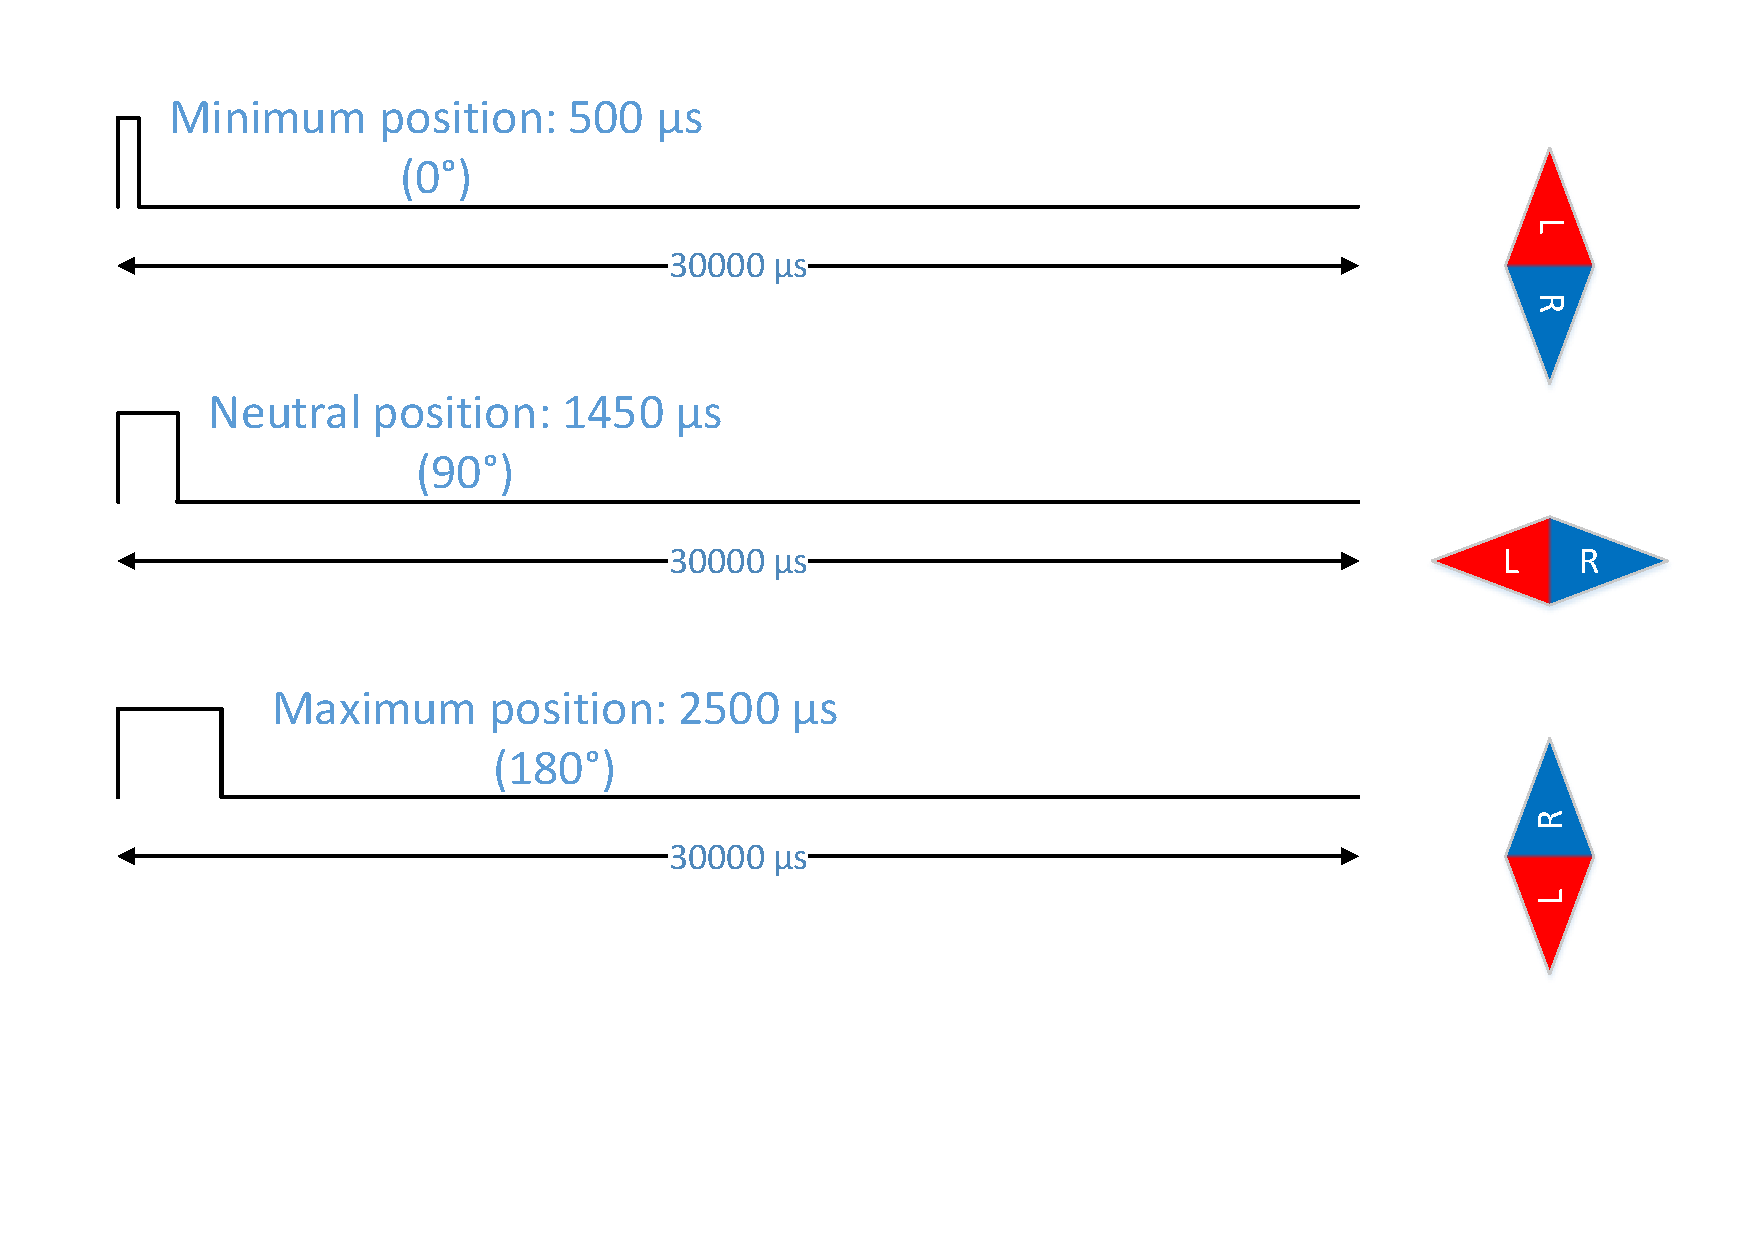
\includegraphics[scale=0.6]{figures/TimeVSangle.pdf}
	\caption{Convertion from PWM to angle by the servo. The figure to the right, shows how the mechanical arm reacts to the PWM signal (Red is left side and blue is right side of the arm). The minimum position is defined at 0°, neutral position at 90° and maximum position at 180°.}
	\label{timeVSangle}
\end{figure}

The servo reacts linearly to the PWM signal and the cycle of the signal is 30000 microseconds \todo{Insert ref to the datasheet}. The indication on which angle the arm is having is took from the minimum position, because it is the smallest PWM signal the servo can use. This position is set to 0°.
 
When the mechanical arm is in neutral position, none of the gears is affected by a braking force. This position is indicated at 90°, as it is turned a quarter of a turn from the minimum position. When the angle is smaller than 90°, the servo will trigger the right brake and begin to slow down the right gear. This position of the arm will not affect the left brake. When the angle is bigger than 90°, the reverse function will happen and the left brake is triggered and the right brake will not be braking the gear.

When the servo brakes on one of the belt, the force, that should be lost in the braking, is transfer to the other belt, by the differential gear system.